\documentclass[CJK]{beamer}
\usepackage{CJKutf8}
\usepackage{beamerthemesplit}
\usetheme{Malmoe}
\useoutertheme[footline=authortitle]{miniframes}
\usepackage{amsmath}
\usepackage{amssymb}
\usepackage{graphicx}
\usepackage{eufrak}
\usepackage{color}
\usepackage{slashed}
\usepackage{simplewick}
\usepackage{tikz}
\usepackage{tcolorbox}
\graphicspath{{../figures/}}
%%figures
\def\lfig#1#2{\includegraphics[width=#1 in]{#2}}
\def\addfig#1#2{\begin{center}\includegraphics[width=#1 in]{#2}\end{center}}
\def\wulian{
\includegraphics[width=0.18in]{emoji_wulian.jpg}}
\def\bigwulian{
\includegraphics[width=0.35in]{emoji_wulian.jpg}}
\def\bye{
\includegraphics[width=0.18in]{emoji_bye.jpg}}
\def\bigbye{
\includegraphics[width=0.35in]{emoji_bye.jpg}}
\def\huaixiao{
\includegraphics[width=0.18in]{emoji_huaixiao.jpg}}
\def\bighuaixiao{
\includegraphics[width=0.35in]{emoji_huaixiao.jpg}}
%% colors
\def\blacktext#1{{\color{black}#1}}
\def\bluetext#1{{\color{blue}#1}}
\def\redtext#1{{\color{red}#1}}
\def\darkbluetext#1{{\color[rgb]{0,0.2,0.6}#1}}
\def\skybluetext#1{{\color[rgb]{0.2,0.7,1.}#1}}
\def\cyantext#1{{\color[rgb]{0.,0.5,0.5}#1}}
\def\greentext#1{{\color[rgb]{0,0.7,0.1}#1}}
\def\darkgray{\color[rgb]{0.2,0.2,0.2}}
\def\lightgray{\color[rgb]{0.6,0.6,0.6}}
\def\gray{\color[rgb]{0.4,0.4,0.4}}
\def\blue{\color{blue}}
\def\red{\color{red}}
\def\green{\color{green}}
\def\darkgreen{\color[rgb]{0,0.4,0.1}}
\def\darkblue{\color[rgb]{0,0.2,0.6}}
\def\skyblue{\color[rgb]{0.2,0.7,1.}}
%%control
\def\be{\begin{equation}}
\def\ee{\nonumber\end{equation}}
\def\bea{\begin{eqnarray}}
\def\eea{\nonumber\end{eqnarray}}
\def\bch{\begin{CJK}{UTF8}{gbsn}}
\def\ech{\end{CJK}}
\def\bitem{\begin{itemize}}
\def\eitem{\end{itemize}}
\def\bcenter{\begin{center}}
\def\ecenter{\end{center}}
\def\bex{\begin{minipage}{0.2\textwidth}
\includegraphics[width=0.6in]{jugelizi.png}\end{minipage}\begin{minipage}{0.76\textwidth}}
\def\eex{\end{minipage}}
\def\chtitle#1{\frametitle{\bch#1\ech}}
\def\bmat#1{\left(\begin{array}{#1}}
\def\emat{\end{array}\right)}
\def\bcase#1{\left\{\begin{array}{#1}}
\def\ecase{\end{array}\right.}
\def\bmini#1{\begin{minipage}{#1\textwidth}}
\def\emini{\end{minipage}}
\def\tbox#1{\begin{tcolorbox}#1\end{tcolorbox}}
\def\pfrac#1#2#3{\left(\frac{\partial #1}{\partial #2}\right)_{#3}}
%%symbols
\def\sone{$\star$}
\def\stwo{$\star\star$}
\def\sthree{$\star\star\star$}
\def\sfour{$\star\star\star\star$}
\def\sfive{$\star\star\star\star\star$}
\def\rint{{\int_\leftrightarrow}}
\def\roint{{\oint_\leftrightarrow}}
\def\stdHf{{\textit{\r H}_f}}
\def\deltaH{{\Delta \textit{\r H}}}
\def\ii{{\dot{\imath}}}
\def\skipline{{\vskip0.1in}}
\def\skiplines{{\vskip0.2in}}
\def\lagr{{\mathcal{L}}}
\def\hamil{{\mathcal{H}}}
\def\vecv{{\mathbf{v}}}
\def\vecx{{\mathbf{x}}}
\def\vecy{{\mathbf{y}}}
\def\veck{{\mathbf{k}}}
\def\vecp{{\mathbf{p}}}
\def\vecn{{\mathbf{n}}}
\def\vecA{{\mathbf{A}}}
\def\vecP{{\mathbf{P}}}
\def\vecsigma{{\mathbf{\sigma}}}
\def\hatJn{{\hat{J_\vecn}}}
\def\hatJx{{\hat{J_x}}}
\def\hatJy{{\hat{J_y}}}
\def\hatJz{{\hat{J_z}}}
\def\hatj#1{\hat{J_{#1}}}
\def\hatphi{{\hat{\phi}}}
\def\hatq{{\hat{q}}}
\def\hatpi{{\hat{\pi}}}
\def\vel{\upsilon}
\def\Dint{{\mathcal{D}}}
\def\adag{{\hat{a}^\dagger}}
\def\bdag{{\hat{b}^\dagger}}
\def\cdag{{\hat{c}^\dagger}}
\def\ddag{{\hat{d}^\dagger}}
\def\hata{{\hat{a}}}
\def\hatb{{\hat{b}}}
\def\hatc{{\hat{c}}}
\def\hatd{{\hat{d}}}
\def\hatN{{\hat{N}}}
\def\hatH{{\hat{H}}}
\def\hatp{{\hat{p}}}
\def\Fup{{F^{\mu\nu}}}
\def\Fdown{{F_{\mu\nu}}}
\def\newl{\nonumber \\}
\def\vece{\mathrm{e}}
\def\calM{{\mathcal{M}}}
\def\calT{{\mathcal{T}}}
\def\calR{{\mathcal{R}}}
\def\barpsi{\bar{\psi}}
\def\baru{\bar{u}}
\def\barv{\bar{\upsilon}}
\def\qeq{\stackrel{?}{=}}
\def\torder#1{\mathcal{T}\left(#1\right)}
\def\rorder#1{\mathcal{R}\left(#1\right)}
\def\contr#1#2{\contraction{}{#1}{}{#2}#1#2}
\def\trof#1{\mathrm{Tr}\left(#1\right)}
\def\trace{\mathrm{Tr}}
\def\comm#1{\ \ \ \left(\mathrm{used}\ #1\right)}
\def\tcomm#1{\ \ \ (\text{#1})}
\def\slp{\slashed{p}}
\def\slk{\slashed{k}}
\def\calp{{\mathfrak{p}}}
\def\veccalp{\mathbf{\mathfrak{p}}}
\def\Tthree{T_{\tiny \textcircled{3}}}
\def\pthree{p_{\tiny \textcircled{3}}}
\def\dbar{{\,\mathchar'26\mkern-12mu d}}
\def\erf{\mathrm{erf}}
\def\const{\mathrm{constant}}
\def\pheat{\pfrac p{\ln T}V}
\def\vheat{\pfrac V{\ln T}p}
%%units
\def\fdeg{{^\circ \mathrm{F}}}
\def\cdeg{^\circ \mathrm{C}}
\def\atm{\,\mathrm{atm}}
\def\angstrom{\,\text{\AA}}
\def\SIL{\,\mathrm{L}}
\def\SIkm{\,\mathrm{km}}
\def\SIyr{\,\mathrm{yr}}
\def\SIGyr{\,\mathrm{Gyr}}
\def\SIV{\,\mathrm{V}}
\def\SImV{\,\mathrm{mV}}
\def\SIeV{\,\mathrm{eV}}
\def\SIkeV{\,\mathrm{keV}}
\def\SIMeV{\,\mathrm{MeV}}
\def\SIGeV{\,\mathrm{GeV}}
\def\SIcal{\,\mathrm{cal}}
\def\SIkcal{\,\mathrm{kcal}}
\def\SImol{\,\mathrm{mol}}
\def\SIN{\,\mathrm{N}}
\def\SIHz{\,\mathrm{Hz}}
\def\SIm{\,\mathrm{m}}
\def\SIcm{\,\mathrm{cm}}
\def\SIfm{\,\mathrm{fm}}
\def\SImm{\,\mathrm{mm}}
\def\SInm{\,\mathrm{nm}}
\def\SImum{\,\mathrm{\mu m}}
\def\SIJ{\,\mathrm{J}}
\def\SIW{\,\mathrm{W}}
\def\SIkJ{\,\mathrm{kJ}}
\def\SIs{\,\mathrm{s}}
\def\SIkg{\,\mathrm{kg}}
\def\SIg{\,\mathrm{g}}
\def\SIK{\,\mathrm{K}}
\def\SImmHg{\,\mathrm{mmHg}}
\def\SIPa{\,\mathrm{Pa}}

\def\courseurl{https://github.com/zqhuang/SYSU\_TD}

\def\tpage#1#2{
\begin{frame}
\begin{center}
\begin{Large}
\bch
热学 \\
第#1讲 #2

{\vskip 0.3in}

黄志琦

\ech
\end{Large}
\end{center}

\vskip 0.2in

\bch
教材:《热学》第二版,赵凯华,罗蔚茵,高等教育出版社
\ech

\bch
课件下载
\ech
\courseurl
\end{frame}
}

\title{Lesson 08 Sad Midterm}
  \author{}
  \date{}
\begin{document}
\tpage{8}{崩溃的期中考试}

\section{Review}

\begin{frame}
\chtitle{上讲内容回顾}
\bch
\bitem
\item{内能是态函数}
\item{热力学第一定律:$\Delta U = A + Q$。}
\item{绝热过程状态方程:$pV^\gamma = \const$ ,其中$\gamma = C_p/C_V = (C_V + \nu R)/C_V$。}
\item{大气的绝热近似:空气中的声速$u_s =\sqrt{\gamma}$;干燥空气垂直温度梯度$\frac{dT}{dz} \approx -10 \SIK/\SIkm$。}
\item{多方过程气体对外做功$A' = -\frac{\nu R}{n-1}\Delta T$ (等温过程$n=1$则需要另算)。}
\item{多方过程热容$C_n =C_V -\frac{\nu R}{n-1}$ (等温过程$C = \infty$)。}
\eitem
\ech
\end{frame}


\begin{frame}
\chtitle{本讲内容}
\bch
\bitem
\item{期中参考答案}
\eitem
\ech
\end{frame}


\begin{frame}
\chtitle{期中考后感}
\bch
\addfig{4}{kaigua.jpg}
\ech
\end{frame}


\begin{frame}
\chtitle{悲剧的主要原因}
\bch
\bmini{0.12}
你们用学历史的方法学物理
\emini
\bmini{0.7}
\addfig{3}{teaching.png}
\emini
\bmini{0.12}
我们用教数学的方法教物理
\emini
\ech
\end{frame}

\begin{frame}
\chtitle{第一题}
\bch
{\blue 
\bitem
\item[(1)]{\blue 叙述热力学第零定律; (10分)}
\item[(2)]{\blue 叙述定体气体温度计和定压气体温度计的工作原理。(10分)}
\eitem
}
\ech
\end{frame}

\begin{frame}
\chtitle{(1)叙述热力学第零定律(10分)}
\bch

{\darkgreen 
在与外界影响隔绝的条件下,如果物体A、B分别与处于{\bf 确定状态}的物体C达到热平衡,则物体A和B也是相互热平衡的。
}

{\small
\bitem
\item{没有提到“外界影响隔绝”不扣分。}
\item{如果没有说明物体C处于确定状态,或者说成A,B处于确定状态,则说明你完全没有理解热力学第零定律,(放水)给8分。}
\item{如果瞎扯了一堆温度热平衡之类的概念,按照相关度给1-7分。}
\eitem
}
\ech
\end{frame}

\begin{frame}
\chtitle{(2)叙述定体气体温度计和定压气体温度计的工作原理(10分)}
\bch
{\darkgreen
定体气体温度计:气体固定体积时压强近似和温度成正比(+5分)。
}
{\small
\bitem
\item{没提到固定体积,扣1分。}
\item{没有提到近似正比,说根据一定关系或者说随着温度升高而压强增大等,扣1分。但如提到理想气体状态方程,或能画出正确的工作原理图,则这1分不扣。}
\eitem
}

{\darkgreen
定压气体温度计:气体固定压强时体积近似和温度成正比(+5分)。
}

{\small
\bitem
\item{没提到固定压强,扣1分。}
\item{没有提到近似正比,说根据一定关系或者说随着温度升高而体积增大等,扣1分。但如提到理想气体状态方程,或能画出正确的工作原理图,则这1分不扣。}
\eitem
}

\ech
\end{frame}


\begin{frame}
\chtitle{第二题}
\bch
{\blue 把摩尔数为$\nu_1$,每个分子质量为$m_1$的理想气体和摩尔数为$\nu_2$,每个分子质量为$m_2$的理想气体混合而成的气体置于容积为$V$,温度为$T$的恒温箱内达到热平衡。两种气体间无化学反应。
\bitem
\item[(1)]{\blue 求混合气体的压强$p$; (5分)}
\item[(2)]{\blue 求混合气体的分子平均速率$\overline{\upsilon}$; (5分)}
\item[(3)]{\blue 求混合气体的分子方均根速率$\upsilon_{\rm rms} $; (5分)}
\item[(4)]{\blue 证明$\upsilon_{\rm rms} > \overline{\upsilon}$。(5分)}
\eitem
}
\ech
\end{frame}

\begin{frame}
\chtitle{(1)求混合气体的压强$p$; (5分)}
\bch
{\darkgreen
两种气体压强分别为
$$ p_1 = \frac{\nu_1 RT}{V}$$
$$ p_2 = \frac{\nu_2 RT}{V}$$
根据道尔顿分压定律
$$p = p_1+p_2 = \frac{(\nu_1+\nu_2)RT}{V}$$
}
{\small
\bitem
\item{答案对即给5分}
\item{多乘,多除$N_A$的,(放水)给4分}
\eitem
}
\ech
\end{frame}

\begin{frame}
\chtitle{(2)求混合气体的分子平均速率$\overline{\upsilon}$; (5分)}
\bch
{\darkgreen
两种气体的分子平均速率分别为
$$ \overline{\upsilon_1} =\sqrt{\frac{8kT}{\pi m_1}},\ \overline{\upsilon_2} =\sqrt{\frac{8kT}{\pi m_2}}$$
第一类分子个数为$N_1 = \nu_1 N_A$,第二类分子个数为$N_2 = \nu_2 N_A$,根据分子平均速率的定义(全部分子的速率之和除以总分子数)
$$\overline{\upsilon} = \frac{\sum \upsilon_1 + \sum \upsilon_2}{N_1+N_2} = \frac{N_1\overline{\upsilon_1}+ N_2\overline{\upsilon_2}}{N_1+N_2} = \sqrt{\frac{8kT}{\pi m_1m_2}}\frac{\nu_1\sqrt{m_2} + \nu_2\sqrt{m_1}}{\nu_1+\nu_2} $$
}
{\small
\bitem
\item{答案对即给5分}
\item{其余情况放水规则:用平均质量或者总质量等,+1分;用正确的平均方法则+3分。写出正确的平均速率+2分,否则若正确写出平均速率积分式,+1分。}
\eitem
}
\ech
\end{frame}


\begin{frame}
\chtitle{(3)求混合气体的分子方均根速率$\upsilon_{\rm rms}$; (5分)}
\bch
{\darkgreen
两种气体的速率平方平均分别为
$$ \overline{\upsilon^2_1} = \frac{3kT}{m_1},\ \overline{\upsilon^2_2} =\frac{3kT}{m_2}$$
第一类分子个数为$N_1 = \nu_1 N_A$,第二类分子个数为$N_2 = \nu_2 N_A$,根据分子方均根速率的定义(全部分子的速率平方之和除以总分子数再开平方)
$$\upsilon_{\rm rms} = \sqrt{\frac{\sum \upsilon^2_1 + \sum \upsilon^2_2}{N_1+N_2}} = \sqrt{\frac{N_1\overline{\upsilon^2_1}+ N_2\overline{\upsilon^2_2}}{N_1+N_2} }= \sqrt{ \frac{3kT}{m_1m_2} \frac{\nu_1m_2 + \nu_2m_1}{\nu_1+\nu_2}} $$
}
{\small
\bitem
\item{答案对即给5分}
\item{其余情况放水规则:用平均质量或者总质量等,+1分;用正确的平均方法则+3分。写出正确的方均根速率+2分,否则若正确写出方均根速率积分式,+1分。}
\eitem
}
\ech
\end{frame}

\begin{frame}
\chtitle{(4)证明$\overline{\upsilon}>\overline{\upsilon}$; (5分)}
\bch
{\darkgreen
根据麦克斯韦分布,显然并非所有分子速率相等。所以$\upsilon-\overline{\upsilon}$不可能全为零,其平方平均大于零。
\bea
0 &<& \overline{\left(\upsilon- \overline{\upsilon}\right)^2} \newl
&=& \overline{\upsilon^2} + \overline{\upsilon}^2 - 2\overline{\upsilon\bar{\upsilon}} \newl 
&=& \overline{\upsilon^2} + \overline{\upsilon}^2 - 2\overline{\upsilon}^2 \newl 
&=& \overline{\upsilon^2} - \overline{\upsilon}^2 
\eea
移项开平方即有
$$ \upsilon_{\rm rms} > \overline{\upsilon}$$

}
{\small
\bitem
\item{任何正确的证明给5分。}
\item{其余情况放水规则:思想正确但因代数化简能力不足而未能完成完整证明的酌情给3-4分。因为前面两问用了平均质量或者总质量,这一问直接根据$3>\frac{8}{\pi}$得出结论,给2分。}
\eitem
}
\ech
\end{frame}

\begin{frame}
\chtitle{第三题}
\bch
{\blue
有一团二维气体被束缚在$xy$平面内运动。气体粒子的速度分布为
$$f(\upsilon_x, \upsilon_y) = A e^{-B\upsilon} \, (B>0),$$
这里速率定义为$\upsilon =\sqrt{\upsilon_x^2+\upsilon_y^2}$。
\bitem
\item[(a)]{\blue 利用速度分布函数归一化条件,用$B$来表示$A$; (5分)}
\item[(b)]{\blue 求速率$\upsilon$的分布函数; (5分)}
\item[(c)]{\blue 求粒子的平均速率$\overline{\upsilon}$(用$B$表示); (5分)}
\item[(d)]{\blue 求在气体中找到一个粒子,其速率大于$2\overline{\upsilon}$的概率。 (5分)}
\eitem
}
\ech
\end{frame}


\begin{frame}
\chtitle{(1)利用速度分布函数归一化条件,用$B$来表示$A$; (5分)}
\bch
{\darkgreen
速度分布函数的归一化条件为
$$\int_{-\infty}^\infty d\upsilon_x \int_{-\infty}^\infty d\upsilon_y\,  A e^{-B\upsilon} = 1$$
转化到极坐标进行积分
$$\int_0^\infty d\upsilon \int_0^{2\pi} d\varphi \, \upsilon \, A e^{-B\upsilon} = 1$$
即
$$2\pi A \int_0^\infty   \upsilon   e^{-B\upsilon} d\upsilon = \frac{2\pi A}{B^2} = 1$$
即
$$ A = \frac{B^2}{2\pi}$$

}
\ech
\end{frame}


\begin{frame}
\chtitle{(2)求速率$\upsilon$的分布函数; (5分)}
\bch
{\darkgreen
在极坐标下的概率元为
$$  A e^{-B\upsilon} \, \upsilon d\upsilon d\varphi$$
对$\varphi$进行积分即得到$\upsilon$的概率密度函数(即速率分布函数)为:
$$F(\upsilon) =  \int_0^{2\pi} d\varphi \, A \upsilon  e^{-B\upsilon} = 2\pi A \upsilon e^{-B\upsilon} = B^2 \upsilon e^{-B\upsilon}$$
}
\ech
\end{frame}

\begin{frame}
\chtitle{(3)求粒子的平均速率$\overline{\upsilon}$(用$B$表示); (5分)}
\bch
{\darkgreen
$$\overline{\upsilon} = \int_0^\infty \upsilon F(\upsilon) d\upsilon = B^2 \int_0^{\infty} \upsilon^2 e^{-B\upsilon} d\upsilon = \frac{2}{B} $$
}
\ech
\end{frame}


\begin{frame}
\chtitle{(4)求在气体中找到一个粒子,其速率大于$2\overline{\upsilon}$的概率。 (5分)}
\bch
{\darkgreen
\bea
P(\upsilon>2\overline{\upsilon}) &=& \int_{2\overline{\upsilon}}^\infty F(\upsilon) d\upsilon \newl
&=& B^2\int_{\frac{4}{B}}^\infty \upsilon e^{-B\upsilon} d\upsilon \newl
&=& -B\left(\left.\upsilon e^{-B\upsilon}\right\vert_{\frac{4}{B}}^\infty - \int_{\frac{4}{B}}^\infty e^{-B\upsilon} d\upsilon \right) \newl
&=& -B\left(-\frac{4}{B}e^{-4} - \frac{1}{B} e^{-4} \right)\newl
&=& 5 e^{-4}
\eea
}
\ech
\end{frame}

\begin{frame}
\chtitle{第四题}
\bch
{\blue 有一密闭的圆柱型气箱,底面积为$S$,高为$L$。箱内充满了温度为$T$的等温单原子气体,共有$N$个原子,每个原子质量为$m$。将圆柱型气箱在地球重力场中竖直摆放。问气体在气箱上端和下端的气压各为多少。(10分)}
\ech
\end{frame}

\begin{frame}
\chtitle{第四题}
\bch
{\darkgreen \small
根据玻尔兹曼分布律,气体分子数密度为
$$n(z) = n_0e^{-\frac{mgz}{kT}}$$
其中$n_0$为箱底的分子数密度,$z$为离箱底的高度。又总分子数可以写成
$$N = \int_0^L n(z) S dz  = \frac{n_0 S kT}{mg} \left(1- e^{-\frac{mgL}{kT}}\right)  $$
故$n_0 = \frac{mgN}{kT S  \left(1- e^{-\frac{mgL}{kT}}\right)}$

底部压强
$$p(0) = n(0) kT =  n_0 kT =  \frac{mgN}{S  \left(1- e^{-\frac{mgL}{kT}}\right)}$$
顶部压强
$$p(L) = n(L) kT = n_0 e^{-\frac{mgL}{kT}} kT =  \frac{mgN}{S  \left(e^{\frac{mgL}{kT}}-1\right)}$$

}
\ech
\end{frame}

\begin{frame}
\bch
{\blue(五)容器中装有处于热平衡的理想气体,温度为$T$,分子数密度为$n$,每个分子质量为$m$。容器外部为真空。在容器上方开一小孔,面积为$A$。如下图所示。
\begin{center}
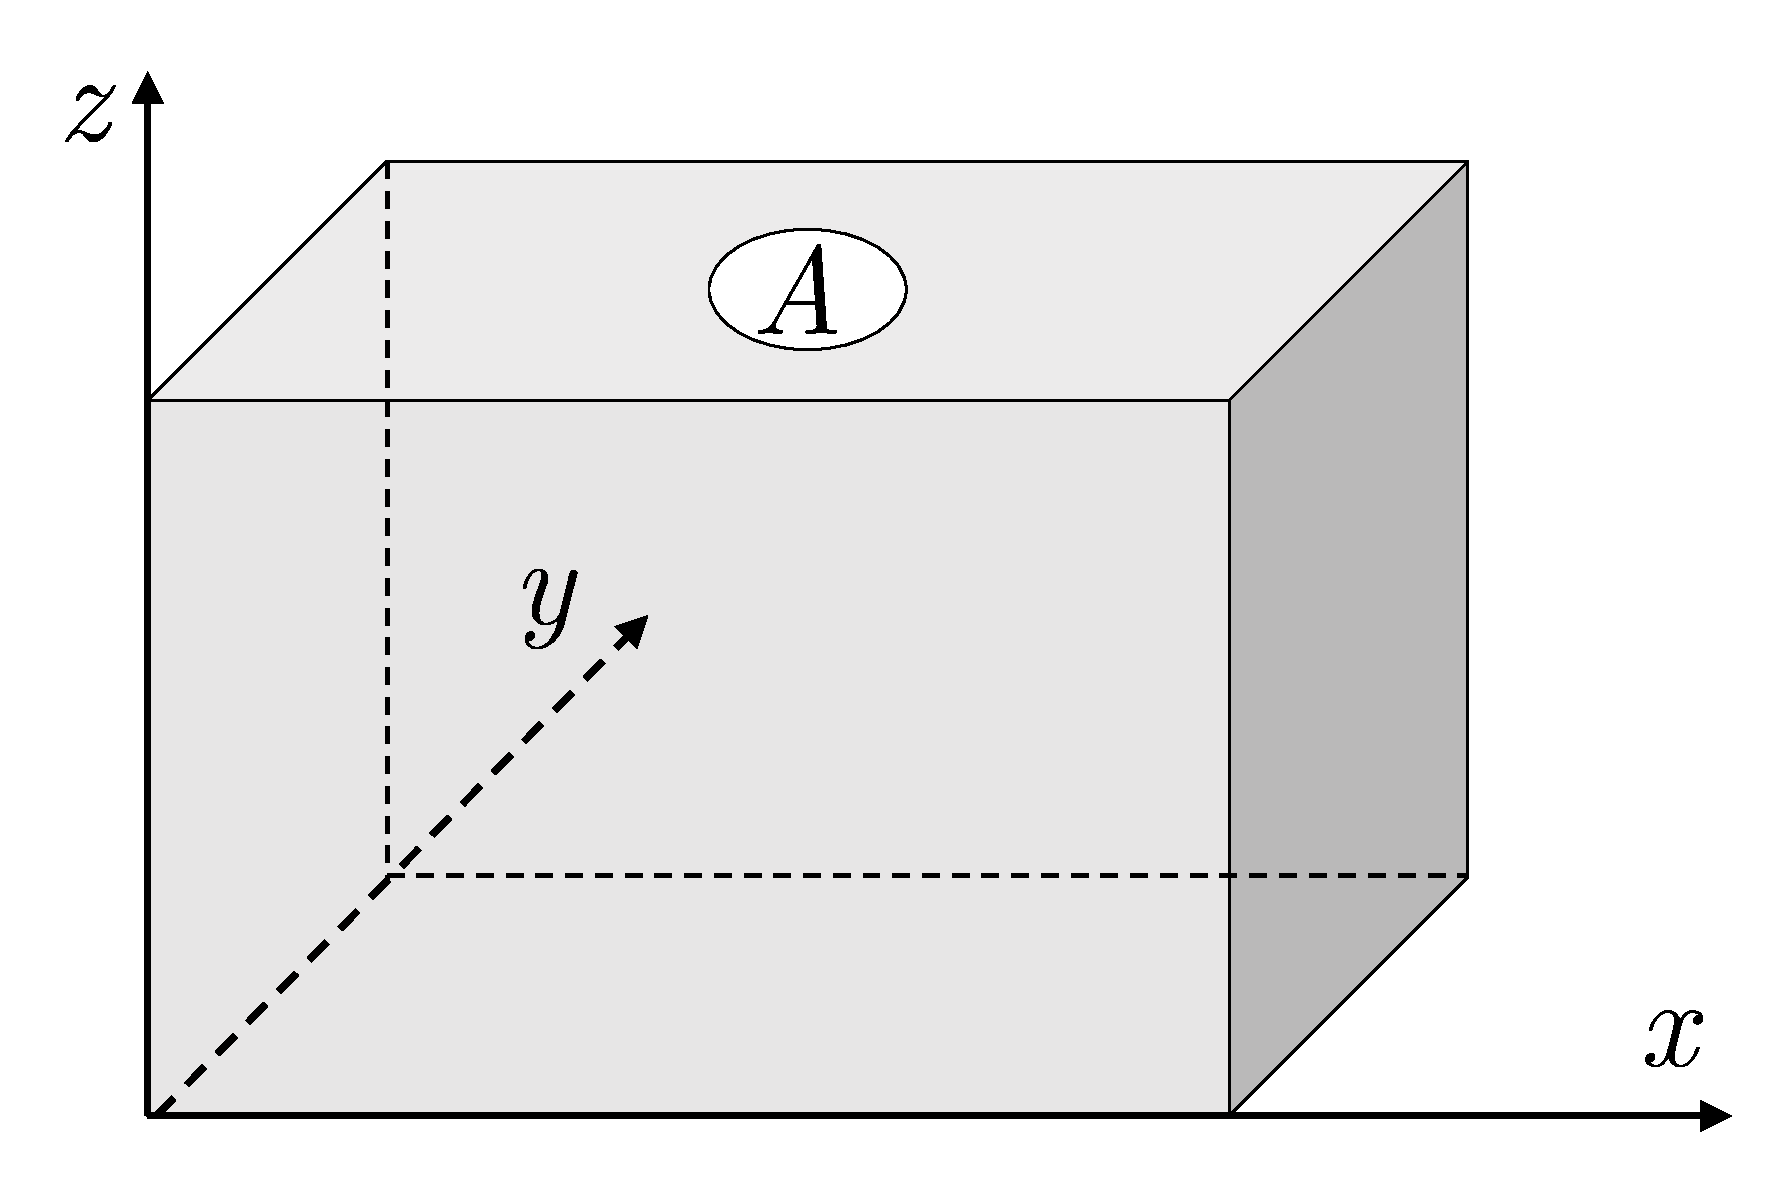
\includegraphics[height=1.3in]{fig1.pdf}
\end{center}
\bitem
\item[(1)]{ \blue 写出容器中分子的速度的分布函数$f(\upsilon_x, \upsilon_y, \upsilon_z)$; (5分)}
\item[(2)]{\blue 证明当$\upsilon_z>0$时,逸出分子的速度的分布函数正比于$\upsilon_z f(\upsilon_x, \upsilon_y, \upsilon_z)$;(10分)}
\item[(3)]{\blue 求逸出分子的速率分布函数$F(\upsilon)$。(5分)}
\eitem
}
\ech
\end{frame}

\begin{frame}
\chtitle{(1) 写出容器中分子的速度的分布函数$f(\upsilon_x, \upsilon_y, \upsilon_z)$; (5分)}
\bch
{\darkgreen

$$f(\upsilon_x, \upsilon_y, \upsilon_z) = \left(\frac{m}{2\pi kT}\right)^{3/2} e^{-\frac{m\upsilon^2}{2kT}}$$
}
\ech
\end{frame}


\begin{frame}
\chtitle{(2)证明当$\upsilon_z>0$时,逸出分子的速度的分布函数正比于$\upsilon_z f(\upsilon_x, \upsilon_y, \upsilon_z)$;(10分)}
\bch
{\small \darkgreen
现在考虑在时间$dt$内,速度在$(\upsilon_x, \upsilon_y, \upsilon_z)$附近的速度体积元$d\upsilon_x d\upsilon_y d\upsilon_z$之内的逸出分子,它必然来自于下图虚线所示的区域:}

\bmini{0.4}
\lfig{1.5}{leak_velocity.jpg}
\emini
\bmini{0.56}
{\darkgreen \small
显然,该区域体积为$S \upsilon_z dt$,其中的分子数为$nS \upsilon_z dt$。又在容器内分子速度在$(\upsilon_x, \upsilon_y, \upsilon_z)$附近的速度体积元$d\upsilon_x d\upsilon_y d\upsilon_z$之内的概率为$f(\upsilon_x, \upsilon_y, \upsilon_z)d\upsilon_x d\upsilon_y d\upsilon_z$。
}
\emini

{\darkgreen \small
因此速度在$(\upsilon_x, \upsilon_y, \upsilon_z)$附近的速度体积元$d\upsilon_x d\upsilon_y d\upsilon_z$之内的逸出分子数为
$$ nS \upsilon_z dt f(\upsilon_x, \upsilon_y, \upsilon_z)d\upsilon_x d\upsilon_y d\upsilon_z \propto \upsilon_z f(\upsilon_x, \upsilon_y, \upsilon_z) d\upsilon_x d\upsilon_y d\upsilon_z $$
根据速度分布函数的定义,上式又正比于逸出分子的速度分布函数乘以$d\upsilon_x d\upsilon_y d\upsilon_z$,故证毕。
}

\ech
\end{frame}

\begin{frame}
\chtitle{(3)求逸出分子的速率分布函数$F(\upsilon)$。(5分)}
\bch
{\darkgreen \small
取球坐标,当$\theta<\frac{\pi}{2}$时,逸出分子的速度分布函数正比于
$$\upsilon^3 \cos\theta e^{-\frac{m\upsilon^2}{2kT}}$$
当$\theta>\frac{\pi}{2}$时,逸出分子的速度分布函数为零。

对$\theta$, $\varphi$积分后,得到速率分布函数
$$ F(\upsilon) \propto \upsilon^3 e^{-\frac{m\upsilon^2}{2kT}}$$
由归一化条件得到

$$ F(\upsilon) = \frac{1}{2} \left(\frac{m}{kT}\right)^2\upsilon^3 e^{-\frac{m\upsilon^2}{2kT}}$$

}
\ech
\end{frame}

\begin{frame}
\bch
{\blue 
(六) 一带小孔(设面积为$A$)的固定隔板把容器分为体积相等(设为$V$)的两部分。整个容器被温度为$T$的恒温热源包围。初始时刻$t=0$,左方装有压强为$P_{0}$,每个分子质量为$m$的理想气体,右方为真空。由于孔很小,虽然板两边分子数都随时间变化,仍可近似认为两边一直都分别处于热平衡。求:
\bitem
\item[(1)]{\blue 初始时刻左方气体在单位时间内减少的分子数;(5分)}
\item[(2)]{\blue 左方气体压强随时间变化的函数形式。(5分)}
\eitem
}
\ech
\end{frame}


\begin{frame}
\chtitle{(1)初始时刻左方气体在单位时间内减少的分子数;(5分)}
\bch
{\darkgreen \small
泻流速率
$$\upsilon_{\rm leak} = \frac{1}{4}\overline{\upsilon} = \sqrt{\frac{kT}{2\pi m}}$$
初始时刻左方分子数密度
$$ n_0 = \frac{P_0}{kT}$$
故单位时间减少的分子数为
$$n_0 A \upsilon_{\rm leak} = \frac{P_0A}{kT}  \sqrt{\frac{kT}{2\pi m}} = \frac{P_0A}{\sqrt{2\pi m kT}}$$
}
\ech
\end{frame}

\begin{frame}
\chtitle{(2) 左方气体压强随时间变化的函数形式。(5分)}
\bch
{\darkgreen \scriptsize
设左边分子数密度为$n$(它是$t$的函数),则由总分子数守恒,右边分子数密度为$n_0-n$。单位时间从左边跑到右边去的分子数为$ N_l = n A \upsilon_{\rm leak}$;从右边跑到左边去的分子为$ N_r = \left(n_0-n\right) A \upsilon_{\rm leak}$。单位时间左边分子数变化量为
$$ V\frac{dn}{dt} = N_r - N_l = \left(n_0 - 2n\right) A \upsilon_{\rm leak}$$
上式可以写成
$$ \frac{1}{n-\frac{n_0}{2}}\frac{dn}{dt} = N_r - N_l = - \frac{2A \upsilon_{\rm leak}}{V}$$
两边从$0$积分到$t$,并利用$t=0$时刻$n=n_0$,即有
$$\left.\ln\left(n-\frac{n_0}{2}\right)\right\vert_0^t=\ln\left(\frac{2n(t)}{n_0} - 1\right)  = - \frac{2A \upsilon_{\rm leak}t}{V}$$
即
$$n(t) = \frac{n_0}{2}\left(1+ e^{- \frac{2A \upsilon_{\rm leak}t}{V} }\right)$$
$$P = n kT =  \frac{P_0}{2}\left(1+ e^{- \sqrt{\frac{2 kT}{\pi m}}\frac{A t}{V}}\right)$$

}
\ech
\end{frame}

\end{document}
